%--------------------
% Packages
% -------------------
\documentclass[11pt,a4paper]{article}
\usepackage[utf8x]{inputenc}
\usepackage[T1]{fontenc}
%\usepackage{gentium}
\usepackage{mathptmx} % Use Times Font
\usepackage{esvect}
\usepackage{mathrsfs}
\usepackage{axodraw2}
\usepackage{braket}

%\usepackage[pdftex]{graphicx} % Required for including pictures
\usepackage[pdftex,linkcolor=black,pdfborder={0 0 0}]{hyperref} % Format links for pdf
\usepackage{calc} % To reset the counter in the document after title page
\usepackage{enumitem} % Includes lists

\frenchspacing % No double spacing between sentences
\linespread{1.2} % Set linespace
\usepackage[a4paper, lmargin=0.1666\paperwidth, rmargin=0.1666\paperwidth, tmargin=0.1111\paperheight, bmargin=0.1111\paperheight]{geometry} %margins
%\usepackage{parskip}

\usepackage[all]{nowidow} % Tries to remove widows
\usepackage[protrusion=true,expansion=true]{microtype} % Improves typography, load after fontpackage is selected

\usepackage{lipsum} % Used for inserting dummy 'Lorem ipsum' text into the template


%-----------------------
% Set pdf information and add title, fill in the fields
%-----------------------
\hypersetup{ 	
pdfsubject = {The Discovery of Dark Matter - NOTES},
pdftitle = {},
pdfauthor = {}
}

%-----------------------
% Begin document
%-----------------------
\begin{document} %All text i dokumentet hamnar mellan dessa taggar, allt ovanför är formatering av dokumentet

\section{On Particle Physics}
\subsection{Standard Model}
\subsubsection{Types of particles}
Particles are split into 2 groups, bosons and fermions (and within these groups they are split even more). The main differenciating factor between these 2 groups is that bosons carry integer spin wheras fermions carry half integer ($\frac{1}{2}, -\frac{3}{2}...$) spin. Also, fermions obey the Pauli exclusion principle (cannot have 2 spin states simultaneously) whereas bosons obey the Bose-Einstein statistics (where bosons can occupy the same spin state).

Within fermions, there consists leptons and quarks, and bosons are your gauge bosons and the Higgs.


\subsection{Cross Sectional Area}
Propagator:
\begin{equation}
    \frac{1}{s} = \frac{1}{q_0^2 - |q|^2} = \frac{1}{{E^{TOT}_{CoM}}^2}
\end{equation}

\subsection{Luminosity}
Luminosity $\mathscr{L}$, is number of collisions per unit area per second (number of events that will be observed), quoted in $cm^{-2}s^{-1}$. A higher luminosity means greater likelihood particles will collide and result in a desired interaction

\subsubsection{Connection with Cross sectional area, $\sigma$}
Luminosity measures how many particles pass through a square centimetre per second. Cross section measures
the likelihood that a desired event will happen. These two are inversely related in that the luminosity times the
cross section gives the number of expected events per second.

rate of reaction, $R = \frac{dN}{dt} = \mathscr{L}\sigma$

see: \url{https://cds.cern.ch/record/2800578/files/Cross%20Section%20and%20Luminosity%20Physics%20Cheat%20Sheet.pdf}

integrated luminosity, $L = \int \mathscr{L} dt$
total number of events, $N = \int (\mathscr{L}\sigma) dt$, with error of $\sqrt{N}$, and accuracy of $\frac{1}{\sqrt{N}}$.

luminosity is proportional to the square of the number of particles in each beam, $n$, the revolution frequency, $f$, number of particles in each beam, $N_1$ and $N_2$, and inversely proportional to the beam cross section $A$.
\begin{equation}
    \mathscr{L} = \frac{n^2 f N_1 N_2}{A}
\end{equation}

\subsubsection{Matrix Element}
Matrix element, $\mathscr{M}^{i, f}$, where $i$ and $f$ are initial and final states respectively, is another way of describing states, as opposed to bra-ket notation. 
\subsection{Feynman Rules}
To obtain the amplitude of an interaction, there are some rules used. For an EM interaction:
\begin{itemize}
    \item Vertex is proportional to the charge
    \item Conservation of E and $\vec{p}$ at each vertex
    \item The propagator: 
        \begin{equation}
            D(q_o, \vec{q}) = \frac{1}{q_0^2 - |\vec{q}|^2 - M + i\Gamma M}
        \end{equation}
        Where $q_0 = \frac{(E^1 _f - E^1 _i)}{c} = \frac{(E^2 _f - E^2 _i)}{c}$
        and $\vec{q} = \vec{p}^1_f - \vec{p}^1_i = \vec{p}^2_f - \vec{p}^2_i$
\end{itemize}
And so the amplitude of the interaction, $\mathscr{A}$ is proportional to:
\begin{equation}
    \frac{e_1 e_2}{q_0^2 - |\vec{q}|^2} = \frac{e_1 e_2}{\frac{(E^1 _f - E^1 _i)}{c} - \vec{p}^1_f - \vec{p}^1_i}
\end{equation}

And we can say that $\mathscr{A} \propto \frac{e^2}{s}$

\begin{figure}[h]
    \centering
    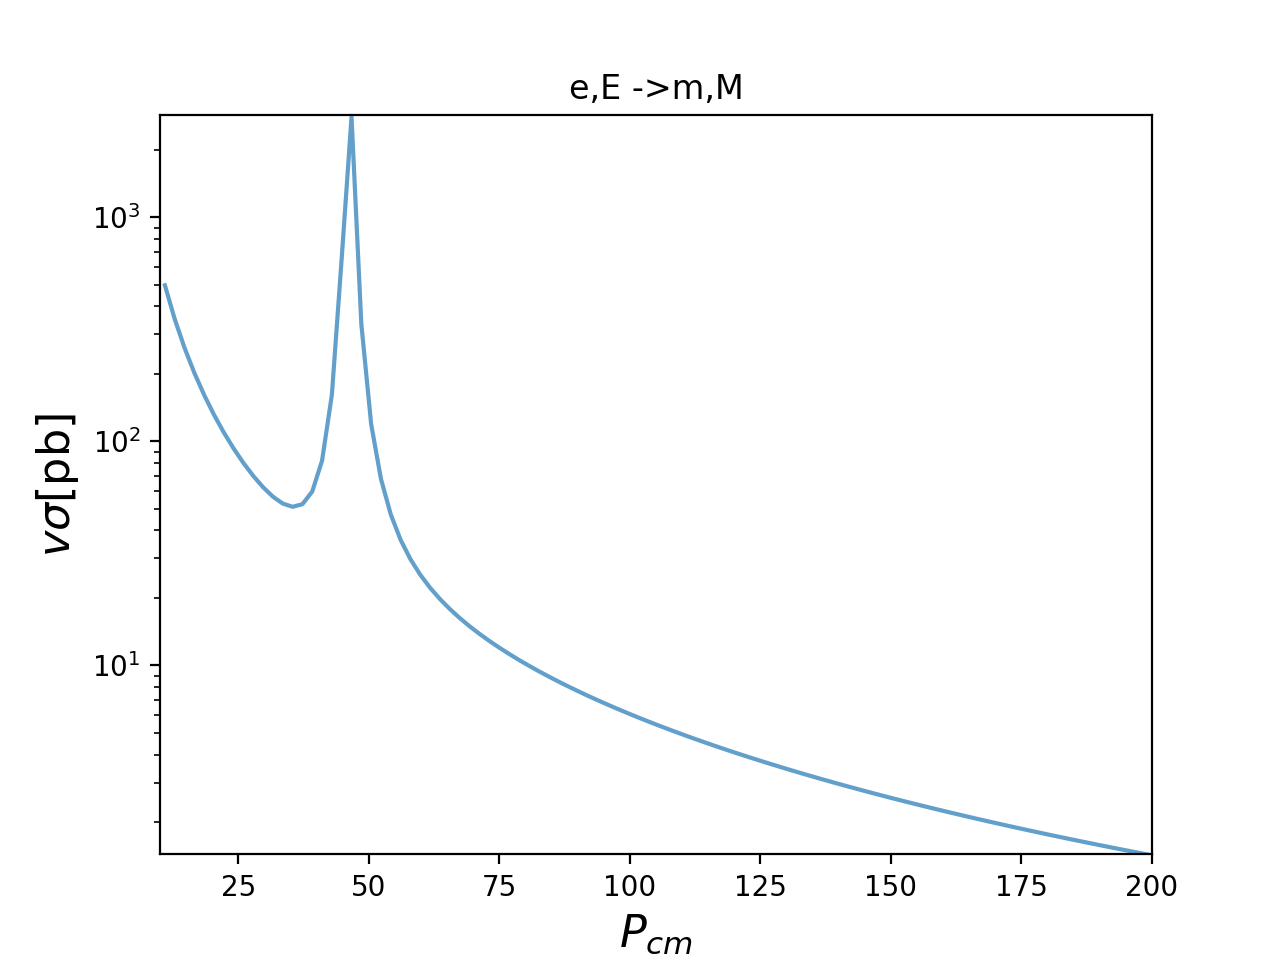
\includegraphics[width=0.5\linewidth]{Documents/Notes/Fig/eE-mM.png}
    \caption{Cross sectional area of interaction between $e^-$, $e^+$ annihilating to give $\mu^+$ $\mu^-$. The resonance peak is the energy of the $Z^0$ boson}
    \label{fig:enter-label}
\end{figure}

\subsection{Interactions}
\subsubsection{Electromagnetic}
Intermediate particle (virtual particle): EM wave, $\gamma$.

Conservation Laws:
\begin{itemize}
    \item E, $\vec{p}$ at each vertex
    \item Charge, Q
    \item Lepton number ($L_{e^-} = +1$, $L_{e^+} = -1$)
    \item Flavour
\end{itemize}

\subsubsection{Strong}
Intermediate particle (virtual particle): Gluon, g

\begin{itemize}
    \item E, $\vec{p}$ at each vertex
    \item Flavour
\end{itemize}
Note: No electric charges in play, and leptons do not interact strongly.

\subsubsection{Weak (Neutral)}
Intermediate particle (virtual particle):

Z boson, $Z^0$
Similar conservation laws to EM:
\begin{itemize}
    \item E, $\vec{p}$ at each vertex
    \item Charge, Q
    \item Lepton number
    \item Flavour
\end{itemize}

\subsubsection{Weak (Charged)}
Intermediate particle (virtual particle): 

W boson, $W^+$ or $W^-$
Conservation laws:
\begin{itemize}
    \item E, $\vec{p}$ at each vertex
    \item Charge, Q
    \item Lepton number
\end{itemize}

\subsection{Feynman Diagrams}
{
\unitlength=1.0 pt
\SetScale{1.0}
\SetWidth{0.7}      % line    size control
\scriptsize    %  letter  size control
{} \qquad\allowbreak
%  diagram # 1
\begin{picture}(96,38)(0,0)
    \ArrowLine(12.0,35.0)(36.0,23.0) 
    \Text(12.0,35.0)[r]{$e$}
    \ArrowLine(36.0,23.0)(12.0,11.0) 
    \Text(12.0,11.0)[r]{$E$}
    \DashLine(36.0,23.0)(60.0,23.0){3.0} 
    \Text(49.0,24.0)[b]{$A$}
    \ArrowLine(60.0,23.0)(84.0,35.0) 
    \Text(84.0,35.0)[l]{$m$}
    \ArrowLine(84.0,11.0)(60.0,23.0) 
    \Text(84.0,11.0)[l]{$M$}
\end{picture} \ 
{} \qquad\allowbreak
%  diagram # 2
\begin{picture}(96,38)(0,0)
    \ArrowLine(12.0,35.0)(36.0,23.0) 
    \Text(12.0,35.0)[r]{$e$}
    \ArrowLine(36.0,23.0)(12.0,11.0) 
    \Text(12.0,11.0)[r]{$E$}
    \DashLine(36.0,23.0)(60.0,23.0){3.0} 
    \Text(49.0,24.0)[b]{$Z$}
    \ArrowLine(60.0,23.0)(84.0,35.0) 
    \Text(84.0,35.0)[l]{$m$}
    \ArrowLine(84.0,11.0)(60.0,23.0) 
    \Text(84.0,11.0)[l]{$M$}
\end{picture} \ 
}

\subsection{Dirac Equation}
The Dirac equation was introduced to solve the problem of negative energy states that arise from the Klein-Gordon equation when a single particle wave function $\phi$ was used. 
To fix this, an equation with first order derivatives in time was introduced. We start with the Hamiltonian:
\begin{equation}
    H_D = \alpha_1 P_1 + \alpha_2 P_2 + \alpha_3 P_3 +\beta m
\end{equation}
Where $P_i$ are the 3 components of the momentum operator $\vec{p}$, $\alpha_i$ and $\beta$ are constants.

We write the operators as their differential counterparts, since we know that:
\begin{equation}
    p^\mu = i\frac{\partial}{\partial t}, 
    (E, \vec{p}) = (i\frac{\partial}{\partial t}, -i\nabla)
\end{equation}

Giving $H_D = i\frac{\partial}{\partial t}$, and $\alpha_1 P_1 + \alpha_2 P_2 + \alpha_3 P_3 = -i\vec{\alpha}\cdot\vec{\nabla}$

The Dirac equation in position space is then 
\begin{equation}
    i\frac{\partial\psi}{\partial t} = (-i\vec{\alpha}\cdot\vec{\nabla} + \beta m)\psi
\end{equation}
\section{Dark Matter}
Initially, universe hot with initial temp unknown (big bang, dont know when and how hot. we know for sure it was above 10MeV, otherwise big bang will not happen). This
should be sufficiently hot to generate protons and neutrons.
strong confidence that there was inflation (big bang was an expansion from a singularity which slowed down over time)
all particles in plasma in thermal equilibrium. energy of plasma -> high enough to produce particles ($E = mc^2$)
assume DM is particles. and DM interact with particles. 

At high enough temps (higher than their mass) they behave relativistic and behave similarly (same number of dof (1-3 factor difference))
universe cooling down, temp drops exponentially ~14 billion years to current day.
at some point the temperature became lower than DM mass, meaning it can annihilate with SM particles (however, there is no reverse process. (freeze out process))
dark matter -> sm particles, no way around. depending on c.s, relic density can be derived. higher rate, the less DM there is.
dm density drops due to annihilation. reaction rate becomes smaller than the rate of expansion of the universe. then DM canot annihilate anymore due to low density. then dm density ~ constant (freeze out)
if DM annihilates too strongly, no relic DM left. If DM reacts too weakly, there will be too little DM, and the universe will be filled with too much DM -> universe closes up
controlled by Boltzmann equation (classical) to know the rate of reaction. 
freeze in - if DM interacts with SM particles weakly, at high temps SM particles and DM will not be in thermal equilibrium (since they react weakly). rarely that SM particles react with DM. 

There are many experiments done that can confirm the existance of DM.

\begin{itemize}
    \item Galactic Rotation Curves - The observed curves do not match the predicted curves due to the fact that the Milky Way is surrounded by DM
    \item CMB (WMAP and PLANCK): Confirmed relic density
    \item Large Scale Structures: Simulation of the formation of galaxies are not possible if DM is not accounted for. Therefore, if there was no DM, the universe would not have formed.
    \item Gravitational Lensing: DM present as an intergalactic medium and plays a role as a gravitational lens (Objects appear to be warped)
    \item Bullet Clusters: Clusters of galaxies collide, DM passes through each other.
\end{itemize}

Now we know that DM exists, a suitable candidate for DM can be considered from the SM. The candidate has to be neutral, colourless, non-baryonic, long-lived (DM life exceeds age of the Universe) and massive (non-relativistic). However, none of the SM particles fit the description. The \textbf{most likely} candidate would be the neutrino, only thing is that it is very light and does not have a long lifetime. This points to the requirement of a new particle to describe DM.

\subsection{Freeze-out}
There comes a point where the energy of particles is lesser than the mass of dark matter mass. This is when the particles stop interacting with each other which result in a phenomenon called freeze-out. Dark matter is then left in the universe which is known as relic dark matter. The density of the dark matter left is called the relic density.

The equation governing the relic density is derived from the Boltzmann equation. The Boltzmann equation is:
\begin{equation}
    \frac{dn}{dt} = -3H_n - <\sigma_a \nu>(n^2 - n^2_{eq})
\end{equation}

Where:
\begin{itemize}
    \item $n$ is the number density of DM
    \item $n_{eq}$ is the dark matter density in thermal equilibrium 
    \item $H$ is the Hubble constant
    \item $<\sigma_a \nu>$ is the thermally averaged cross-section of annihilation
\end{itemize}

$n^2$ comes from the annihilation process of SM particles to DM, whereas $n_{eq}^2$ comes from annihilation of DM particles to SM particles. The Boltzmann equation can be solved to derive the thermal relic density equation, $\Omega$. We set $<\sigma_a \nu>n = H$:
\begin{equation}
    n_f \approx (m_X T_f)^{3/2}e^{\frac{-m_X}{T_f}} \approx \frac{{T_f}^2}{m_{Planck}<\sigma_a \nu>}
\end{equation}

Where now:
\begin{itemize}
    \item $m_X$ is DM mass
    \item $T_f$ is the temperature at freeze out
    \item $m_{Planck}$ is Planck mass
\end{itemize}

The exponential term is a constant denoted as $x_f$, which is $\approx20$.

The DM relic density, usually denoted as $\Omega_X$ is:
\begin{equation}
    \Omega_X = \frac{m_X n_0}{\rho_c} = \frac{m_X T_0^3}{\rho_c}\frac{n_0}{T_0^3} \approx \frac{m_X T_0^3}{\rho_c}\frac{n_0}{T_f^3} \approx \frac{x_f T_0^3}{\rho_c m_{Planck}}<\sigma_A\nu>^{-1}
\end{equation}

Where $\rho_c$ is critical density.

\section{Detection of Dark Matter}
\subsection{Direct}
Underground Dirac detection
\subsection{Indirect}
Collider search, where:
\begin{itemize}
    \item $E = mc^2$, can derive mass of DM from energy of collider
    \item A visible particle is recoiled by an invisible particle
    \item Missing momenta can deduce mass of Dark matter
\end{itemize}

\section{Dark Matter Relic Density}
DM Relic Density, usually 

\section{i2HDM}
\begin{itemize}
    \item higgs field before EWSB:
        \begin{equation}
            \Phi_H =
                \begin{pmatrix}
                    {\phi_1 + i\phi_2} \\
                    {\phi_3 + i\phi_4}
                \end{pmatrix}
        \end{equation}
    \item after EWSB, vev obtained:
        \begin{equation}
            \braket{\Phi_H} =
                \begin{pmatrix}
                    {0} \\
                    {\frac{v}{\sqrt{2}}}
                \end{pmatrix}
        \end{equation}
    \item $\phi_{1, 2, 3}$ give mass to $W^\pm$ and $Z_0$ bosons due to Lagrangian. (via higgs mechanism)
    \item 3 out of 4 dof become mass and last dof is the higgs particle itself.
    \item yukawa interactions then give masses to the fermions via Higgs field (because there is vev)
\end{itemize}

\section{parameter search}
\begin{itemize}
    \item collider energy 13.6TeV
    \item pp -> DM interaction
    \item set f(x,Q)(proton density function) to ensure correct numbers
    
\end{itemize}
\section{CalcHEP/microOMEGAS Notes}
\subsection{microOMEGAS}
\begin{verbatim}main_random_scan.c\end{verbatim} does random scan (log-scale of 10000 points) over parameters with min/max values in lines 104-107, and writes file \begin{verbatim}scan.dat\end{verbatim} with parameters below:
\begin{itemize}
    \item $M_{Z_0}<m_{h_1} + m_{h_2}$ for param space to survive
    \item $\Omega h^2$ $\rightarrow$ $\Omega h^2$ protonSI $\rightarrow$ DM Scattering cross-section
    \item $Pval_{DD}$ - P-value of DM direct detection (DD). if $Pval < 0.1$, point excluded by DM DD at $90\%$ confidence level. name = $e^{DD}$ parameter. this is the probablility that the DM will be directly detected. Since DM cannot be directly detected, if $Pval_{DD} < 0.1$, can reject.
    \item CMB ID = DM limit from CMB constraints - if CMB ID > 1, point excluded by $90\%$ CL by constraints
    \item $Br(H\rightarrow DM, DM)$ Higgs branching ratio (invisible Higgs decay) in code val <0.1 - see latest papers for info.
\end{itemize}
\subsection{plotting}
run \begin{verbatim}gzip ./scan.dat\end{verbatim} to be able to allow pandas to read data.
\begin{itemize}
    \item apply selection criteria ($\Omega h^2$ < 1), but apply planck constraints in final
    \item plots in $m_{D_1}-\lambda_{345}$ plane. color map reflects relic density
    \item adjustments need to be done.
\end{itemize}
\ref{test2002}
\bibliography{Documents/Notes/notes_ref}
\end{document}

